\documentclass[a4paper]{article}

% font stuff
\usepackage{fouriernc}
\usepackage[T1]{fontenc}

\usepackage{amsmath}
\usepackage{amssymb}
\usepackage{amsthm}
\usepackage[retainorgcmds]{IEEEtrantools}
\usepackage{enumitem} % no space between enum lists

\usepackage{tikz}
\usetikzlibrary{positioning}
\usetikzlibrary{matrix}


\newcommand{\below}{\sqsubseteq}
\newcommand{\arr}{\rightarrow}
\newcommand{\todo}[1]{\smallskip \noindent \emph{todo: #1} \smallskip}
%\newcommand{\todo}[1]{}
\newcommand{\semantics}[1]{\llbracket #1 \rrbracket}
\newcommand{\lub}{\bigsqcup}
\newcommand{\set}[1]{\{\,#1\,\}}
% partial function arrow
% https://tex.stackexchange.com/questions/47142/how-to-tex-an-arrow-with-vertical-stroke
\newcommand{\pfun}{\mathrel{\ooalign{\hfil$\mapstochar\mkern5mu$\hfil\cr$\to$\cr}}}
\newcommand{\isdefined}{\!\downarrow}
\newcommand{\bbN}{\mathbb{N}}
\newcommand{\aand}{\ \wedge \ }


% They all use the same counter, reset at section boundaries
% This gives a running number:
% Section 1
%   Theorem 1.1
%   Definition 1.2
%   Lemma 1.3
% Section 2
%   Definition 2.1
%   Lemma 2.2
%   ...
\newtheorem{definition}{Definition}[section]
\newtheorem{theorem}[definition]{Theorem}
\newtheorem{proposition}[definition]{Proposition}
\newtheorem{lemma}[definition]{Lemma}
\newtheorem{corollary}[definition]{Corollary}

\begin{document}

\title{Thesis}
\author{Markus Klinik}
\maketitle

\begin{abstract}

Abstract

\end{abstract}

\section{Introduction}

Introduction

\todo{fix location of qed signs}

\section{Domain Theory}

\todo{The section on domains in \cite{Gunter1992} is based on his paper with
Scott from 1990}

\begin{definition}

Let $D$ be a poset, $S \subseteq D$. The \emph{least upper bound} (``lub'') of
$S$ is an element $x \in D$ such that:

\begin{equation} \label{eqnLub1}
\forall y \in S \ldotp y \below x
\end{equation}
\begin{equation} \label{eqnLub2}
\forall z \in D \ldotp (\forall y \in S \ldotp y \below z) \implies x \below z
\end{equation}

The lub of S, if it exists, is denoted interchangeably by
\begin{IEEEeqnarray*}{rCl}
\lub S = \lub_{x \in S} x = \lub \set{x \mid x \in S}
\end{IEEEeqnarray*}

\end{definition}


Line (\ref{eqnLub1}) states that the lub is above all elements: it is an upper
bound, and (\ref{eqnLub2}) states that the lub is below any other upper bound:
it is the least such. If a lub exists, it is unique. It is therefore justified
to call it \emph{the} lub.


\begin{definition}

A \emph{chain} in a poset is a linearly ordered subset.

\end{definition}


\begin{definition}

Let $D$ be a poset. A set $S \subseteq D$ is \emph{directed} iff every finite
$P \subseteq S$ has an upper bound in $S$.

\end{definition}


In literature on domain theory and semantics of programming languages, one
encounters three different definitions of complete partial orders.  There is
chain-completeness \cite{Moschovakis1994}, directed-completeness
\cite{DaveyPriestly1990}, \cite{Gunter1992}, and $\omega$-sequence-completeness
\cite{Allison1986}, \cite{Winskel1993}, \cite{BarrWells1990}. Abramsky and Jung
\cite{Abramsky1994} have a short discussion on the equivalence of these
definitions, but refer to further literature for proofs. The proof given here
occurs as an exercise in Davey and Priestly \cite{DaveyPriestly1990}.


\begin{definition} \label{defCpoDirectedComplete}

A directed-complete partial order, \emph{dcpo}, is a partial order where every
directed set has a least upper bound.

\end{definition}


\begin{definition} \label{defCpoChainComplete}

A chain-complete partial order, \emph{ccpo}, is a partial order where every chain
has a least upper bound.

\end{definition}


\begin{definition} \label{defCpoOmegaSequenceComplete}

An $\omega$-sequence-complete partial order, \emph{$\omega$-cpo}, is a partial
order where every non-decreasing sequence of elements $x_0 \below x_1 \below x_2
\below \ldots $ has a least upper bound.

\end{definition}


\begin{proposition} \label{propDefinitionsAreEquivalent}

These three definitions are equivalent.

\end{proposition}

This equivalence justifies simply talking about \emph{complete partial orders},
or \emph{cpos}. We use the definitions interchangeably, whichever is most handy
in a given situation.

For proposition \ref{propDefinitionsAreEquivalent} we give a round-robin proof,
of which two implications are fairly simple. The third implication is a bit more
involved, and requires the axiom of choice. We give a proof for the countable
case here because it is illustrative, and refer to the literature for the
uncountable case. \todo{refer to the literature}


\begin{proof}

$\ref{defCpoDirectedComplete} \implies \ref{defCpoChainComplete}$: Every chain
is a directed set.

$\ref{defCpoChainComplete} \implies \ref{defCpoOmegaSequenceComplete}$:
The image of a non-decreasing $\omega$-sequence is a chain.

$\ref{defCpoOmegaSequenceComplete} \implies \ref{defCpoDirectedComplete}$: Let
$D$ be an $\omega$-cpo as in definition
\ref{defCpoOmegaSequenceComplete}, let $S = \set{x_0, x_1, x_2, \ldots}
\subseteq D$ be countable and directed. For each finite $F \subseteq S$, let
$u(F)$ be an upper bound of $F$ in $S$.  Construct a sequence of sets $P_n
\subseteq S$ as follows,
\begin{IEEEeqnarray*}{rCl}
P_0 & = & \set{x_0} \\
P_{n+1} & = & P_n \cup \set{u(P_n \cup y_n), y_n}
\end{IEEEeqnarray*}

where $y_n$ is the $x_i \in S\backslash P_n$ with the smallest possible $i$.

Every $P_n$ is directed: $P_0$ certainly is, and any finite subset of $P_{n+1}$
has $u(P_n \cup y_n) \in P_{n+1}$ as upper bound.  As every $P_n$ is finite and
directed, taking its lub is justified.

Consider the $\omega$-sequence $Q$ = $\set{\lub P_n}_{n \in \bbN}$. For
all $n$, we have $P_n \subseteq P_{n+1}$ and thus $\lub P_n \below \lub
P_{n+1}$, so $Q$ is non-decreasing, and therefore has a lub $z$.  Each $x \in S$
eventually occurs in some $P_n$, and we have $x \below \lub P_n \below z$, so
$z$ is an upper bound of $S$. Any upper bound $z'$ of $S$ is also an upper bound
of $Q$, and therefore $z \below z'$, i.e. $z$ is the lub of $S$.

\end{proof}


The complication in the third implication comes from the fact that a directed
set doesn't need to be linearly ordered. Every directed set does however contain
a chain which threads through the whole set, eventually rising above all
elements. The lub of the chain is then the lub of the directed set.

\subsection{The Category Cppo}


\begin{definition}

A cpo $D$ is \emph{pointed} iff it has a bottom element $\bot$ which satisfies
$\forall d \in D \ldotp \bot \below d$. Such a pointed cpo is called
\emph{cppo}.

\end{definition}

\begin{definition}

Let $C$, $D$ be partial orders. A function $f : C \arr D$ is \emph{monotone} iff
it is order preserving, that is for all $x, y \in C$,
\begin{IEEEeqnarray*}{rCl}
  x \below y \implies f(x) \below f(y)
\end{IEEEeqnarray*}

\end{definition}

\begin{definition}

Let $C$, $D$ be cpos. A function $f : C \arr D$ is \emph{continuous} iff it
is monotone and preserves lubs, that is for all chains $P \subseteq C$,
\begin{IEEEeqnarray*}{rCl}
  f(\lub_{x \in P} x) = \lub_{x \in P} f(x)
\end{IEEEeqnarray*}

\end{definition}

Note that if a function preserves lubs, it is monotone,
\begin{IEEEeqnarray*}{rCl}
  x \below y \implies
  y = \lub \set{x, y} \implies
  f(y) = f(\lub \set{x, y}) = \lub \set{f(x), f(y)} \implies
  f(x) \below f(y)
\end{IEEEeqnarray*}

but in a proof of continuity of a function $f$, we usually need to prove
monotonicity as a first step, so that for a chain $P$, $\set{f(x) \mid x \in P}$
is again a chain. This motivates the inclusion of
monotonicity in the definition of continuity.


\begin{lemma}

The identity function is continuous.

\end{lemma}

\begin{proof}

Let $P \in C$ be a chain. Then
\begin{equation*}
id(\lub P) = \lub P = \lub_{x \in P} id(x)
\end{equation*}

\end{proof}


\begin{lemma}

Composition of two continuous functions is continuous.

\end{lemma}

\begin{proof}

Let $f : C \arr D$, $g : D \arr E$ be continuous. Let $P \subseteq C$ be a
chain. Then
\begin{IEEEeqnarray*}{rCl}
(g \circ f)(\lub P) & = & g(f(\lub_{x \in P} x)) \\
  & = & g( \lub_{x \in P} f(x) ) \\
  & = & \lub_{x \in P} g(f(x)) \\
  & = & \lub_{x \in P} (g \circ f)(x)
\end{IEEEeqnarray*}

\end{proof}


\begin{corollary}

The complete pointed posets, together with continuous functions between them form
a category.  This category is called Cppo.

\end{corollary}


\begin{definition}

A category has the \emph{fixpoint property} iff for all objects $A$ and arrows
$f : A \arr A$ there exists an arrow $Y(f) : 1 \arr A$ such that $Y(f) = f
\circ Y(f)$.

\end{definition}


\begin{theorem} \label{thmFixpoint}

Cppo has the fixpoint property. In fact, every continuous function on a cppo has
a unique least fixpoint.

\end{theorem}

\begin{proof}

Let $D$ be a cppo, $f : D \arr D$ a continuous function. We have to show that
there exists an element $x \in D$ such that $x = f(x)$. Consider the set
\begin{equation*}
F = \set{f^n(\bot) \mid n \in \bbN}.
\end{equation*}
This set is a chain, because for $n = 0$
we have $f^0(\bot) = \bot \below f(\bot)$. Now assume that $f^n(\bot) \below
f^{n+1}(\bot)$. Then $f(f^n(\bot)) \below f(f^{n+1}(\bot))$, so $f^{n+1}(\bot)
\below f^{n+2}(\bot)$. Because $F$ is a chain and $D$ a cppo, $F$ has a lub $x =
\lub F$.  We calculate:
\begin{IEEEeqnarray*}{rCl}
f(x) & = & f(\lub F) \\
     & = & \lub f(F) \IEEEyesnumber \label{lineFContinuous} \\
     & = & \lub \set{ f(f^n(\bot)) \mid n \in \bbN } \\
     & = & \lub \set{ f^{n+1}(\bot) \mid n \in \bbN } \\
     & = & \lub \set{ f^n(\bot) \mid n \in \bbN }
           \IEEEyesnumber \label{lineLubLeastElement} \\
     & = & \lub F = x
\end{IEEEeqnarray*}
Line (\ref{lineFContinuous}) is because $f$ is continuous, and line
(\ref{lineLubLeastElement}) is because omitting the least element in a chain
doesn't affect the lub.

To see that $x$ is the least fixpoint, let $y = f(y)$ be a fixpoint of $f$. We
have:
\begin{IEEEeqnarray*}{rCl}
\bot \below y & \implies & f(\bot) \below f(y) = y \\
 & \implies & \forall n \in \bbN \ldotp f^n(\bot) \below y \\
 & \implies & y \text{ is an upper bound of F} \\
 & \implies & \lub F = x \below y
\end{IEEEeqnarray*}

\end{proof}

This is the well-known fixpoint theorem, which is sometimes attributed to
Tarski, sometimes to Kleene, but while they both knew the result, its actual
origin seems to be lost in time \cite{Lassez1982}. The formulation given here
is due to Huwig \cite{Huwig1990}.


\begin{lemma} \label{lemCppoTerminalObject}
Cppo has a terminal object.
\end{lemma}

\todo{proof}

\begin{lemma} \label{lemCppoBinaryProducts}
Cppo has binary products.
\end{lemma}

\todo{proof}

\begin{lemma} \label{lemCppoExponentials}
Cppo has exponentials.
\end{lemma}

\todo{proof}

\begin{corollary}
Cppo is cartesian closed.
\end{corollary}


\begin{definition}
A category is \emph{trivial} iff it has exactly one object $A$ and one arrow
$f : A \arr A$, the identity.
\end{definition}

\begin{proposition} \label{propCCCNoFixpointInitialObject}
Any CCC with the fixpoint property and initial object is trivial.
\end{proposition}

\begin{proposition} \label{propCCCNoFixpointCoproducts}
Any CCC with the fixpoint property and binary coproducts is trivial.
\end{proposition}

Propositions \ref{propCCCNoFixpointInitialObject} and
\ref{propCCCNoFixpointCoproducts} are due to Huwig \cite{Huwig1990}, and
demonstrate that if we want to use Cppo as model for programming languages, we
won't get interpretations for sum types that correspond to categorical
coproducts. Nevertheless, we have a similar construction that serves our
purpose.

\todo{what's wrong with separated sums?}

\begin{definition} \label{defCoalescedSum}
For objects $A$, $B$ in Cppo, define the \emph{coalesced sum} $A \oplus B$ as
the disjoint union of $A$ and $B$ where we identify the bottom elements.
\end{definition}

\begin{proposition}
If $A, B$ are cppos, then $A \oplus B$ is a cppo.
\end{proposition}

\todo{proof, show how the order is imposed on A+B}

The injections $\kappa_0 : A \arr A \oplus B$ and $\kappa_1 : B \arr A \oplus B$
are defined in the obvious way.

\begin{equation*}
\kappa_0(a) = \left\{
  \begin{array}{rcl}
   (0,a)             & \text{if} & a \not= \bot_A \\
   \bot_{A \oplus B} & \text{if} & a = \bot_A
  \end{array}
\right.
\end{equation*}

\begin{equation*}
\kappa_1(b) = \left\{
  \begin{array}{rcl}
   (1,b)             & \text{if} & b \not= \bot_B \\
   \bot_{A \oplus B} & \text{if} & b = \bot_B
  \end{array}
\right.
\end{equation*}

\todo{$\kappa_0$ and $\kappa_1$ are continuous}

An element $x \in A \oplus B$ \todo{justify notation $x = \kappa_0(a)$}

If $A, B, D$ are cppos and $f : A \arr D$, $g : B \arr D$ continuous functions,
define $[f,g] : A \oplus B \arr D$ as

\begin{equation*}
[f,g](x) = \left\{
  \begin{array}{rcl}
   f(a)     & \text{if} & x = \kappa_0(a) \\
   g(b)     & \text{if} & x = \kappa_1(b) \\
   \bot_{D} & \text{if} & x = \bot_{A \oplus B}
  \end{array}
\right.
\end{equation*}

Note that $[f,g]$ is a strict function while $f$ and $g$ don't need to be
strict.  Therefore, the usual coproduct diagram (Figure
\ref{figCoproductDiagram}) need not commute. Still, $[f,g]$
is continuous. \todo{proof}

\begin{figure}[ht]
\begin{center}
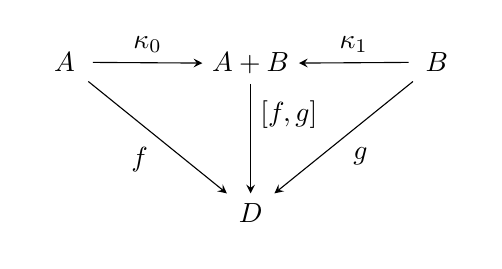
\begin{tikzpicture}[scale=1.2]
\matrix (m) [matrix of math nodes,row sep=4em,column sep=4em,minimum width=2em]
  {
     A & A + B & B \\
     {} & D & {} \\
  };
  \path[-stealth]
    (m-1-1) edge node [below left] {$f$} (m-2-2)
            edge node [above] {$\kappa_0$} (m-1-2)
    (m-1-2) edge node [above right] {$[f,g]$} (m-2-2)
    (m-1-3) edge node [above] {$\kappa_1$} (m-1-2)
            edge node [below right] {$g$} (m-2-2)
    ;
\end{tikzpicture}
\end{center}
\caption{The usual coproduct diagram} \label{figCoproductDiagram}
\end{figure}


\begin{proposition}

For a fixed $D$, the object mapping $L_D : A \mapsto A \oplus D$ extends to a
functor.  Symmetrically for $R_D : A \mapsto D \oplus A$, and we have for all $f
: A \arr A'$ and $g : B \arr B'$, $L_B(f) \circ R_A(g) = R_A(g) \circ L_B(f) : A
\oplus B \arr A' \oplus B'$.  Therefore $\oplus : \text{Cppo} \times \text{Cppo}
\arr \text{Cppo}$ is a bifunctor.

\end{proposition}

\todo{proof}

So while $\oplus$ is not the categorical coproduct, it is still a useful
construction and we can work with it as long as we keep in mind that $[f,g]$
doesn't have the universal mapping property.

This sets up the stage for our following considerations.

\section{Fixpoint Semantics for Recursive Functions}

Using the constructions seen so far, we can show that certain recursive
functions are well-defined. This is the central idea of Scott's fixpoint
semantics for recursive programs, but it can also be employed for mathematical
purposes that don't concern programming.

First, we look at the factorial function, as it is a simple example that nicely
demonstrates the technique at work.

\todo{cite critique 1 in Arbib and Manes for the factorial example}

\begin{lemma} \label{lemPartialFunctionSpaceCppo}

Let $A, B$ be sets. The set of partial functions from $A$ to $B$, denoted
$[A \pfun B]$, is a cppo.

\end{lemma}

\begin{proof}

Let $f, g : A \pfun B$. Define $f \below g$ iff $f \subseteq g$, where we
consider $f$ and $g$ as their underlying graphs.

The totally undefined function $\emptyset = \bot$ is an element of $[A \pfun B]$
and satisfies $\bot \below g$ for all $g$.

If $F$ is a chain of functions, consider $\bigcup F$, the union of the graphs of
all functions in $F$. We have: if $f \in F$ then $f \subseteq \bigcup F$, so $f
\below \bigcup F$.  In other words $\bigcup F$ is an upper bound of $F$.

Furthermore if $g$ is an upper bound of $F$ then $\forall f \in F \ldotp f
\below g$, so $\bigcup F \below g$. In other words $\bigcup F$ is the lub of $F$
and it is justified to write $\lub F$

\end{proof}


The definition of $f \below g$ is equivalent to the following formula, which is
less easy to read, but lends itself better to proofs.
\begin{equation*}
\forall n \in \bbN \ldotp f(n)\isdefined \implies g(n)\isdefined\
\wedge\ f(n) = g(n)
\end{equation*}
Where $f(n)\isdefined$ is to be read as ``$f$ is defined at $n$''.

The following two lemmas are always useful for proving continuity.

\begin{lemma} \label{lemMonotoneAlwaysBelowLub}
Let $A, B$ be cpos, $f : A \arr B$ be a monotone function, and $C \subseteq A$
be a chain in A. Then $\lub f(C) \below f(\lub C)$.
\end{lemma}

\begin{proof}
We have:
\begin{IEEEeqnarray*}{rCl}
           && \forall a \in C \ldotp a \below \lub C \\
 & \implies & \forall a \in C \ldotp f(a) \below f(\lub C) \\
 & \implies & f(\lub C) \text{ is an upper bound of } f(C) \\
 & \implies & \lub f(C) \below f(\lub C)
\end{IEEEeqnarray*}
\end{proof}


\begin{lemma} \label{lemMonotoneIsContinuousFinite}
Let $A, B$ be cpos, $f : A \arr B$ be a monotone function, and $C \subseteq A$
be a finite chain in $A$. Then $f(\lub C) = \lub f(C)$.
\end{lemma}

\begin{proof}
We have $\lub C \in C$, because $C$ is finite. Therefore $f(\lub C) \in f(C)$,
and thus $f(\lub C) \below \lub f(C)$. Lemma \ref{lemMonotoneAlwaysBelowLub}
gives the converse direction.
\end{proof}




\begin{proposition} \label{propFactorialExists}

There exists a function $f : \bbN \arr \bbN$ such that
\begin{IEEEeqnarray}{rCl}
f(0) & = & 1 \label{eqnFactorial1} \\
f(n) & = & n \cdot f(n - 1) \quad\text{if}\ \ n > 0 \label{eqnFactorial2}
\end{IEEEeqnarray}

\end{proposition}

Proposition \ref{propFactorialExists} can be rephrased in different ways: the
recursive definition of the factorial function is not vacuous; it is not a
circular definition; it does not lead to infinite regress.

\todo{
That's interesting. In our case (see far below) we have at some point
$\pi(\_^\omega) = \pi(\kappa_1(\_^\omega)) = \pi(\_^\omega)$, a genuine circle
in the definition.  Yet we argue that the definition is not vacuous. What to
make of that? We surely have $\pi(\_^\omega)\!\uparrow$, $\pi(\_^\omega) = \bot$
so that's the ejection seat.
}

\begin{proof}
From \ref{lemPartialFunctionSpaceCppo} we know that $[\bbN \pfun
\bbN]$ is a cppo. Consider the function

\begin{equation*}
\varphi(g) = n \mapsto \left\{
  \begin{array}{lcl}
   1          & \text{if} & n = 0 \\
   n \cdot g(n-1) & \text{if} & n > 0
  \end{array}
\right.
\end{equation*}

$\varphi$ is not defined recursively, so it certainly is a function $[\bbN
\pfun \bbN] \arr [\bbN \pfun \bbN]$. If we can show that
$\varphi$ is continuous, then it is an arrow in Cppo, so by theorem
\ref{thmFixpoint} it has a fixpoint $f$ such that
\begin{IEEEeqnarray}{rCl}
f = \varphi(f) \label{eqnFactorialFixpoint}
\end{IEEEeqnarray}

Using equation (\ref{eqnFactorialFixpoint}) we proceed to show that the required
equations (\ref{eqnFactorial1}) and (\ref{eqnFactorial2}) hold.
\begin{IEEEeqnarray*}{rCl}
f(0) & = & \varphi(f)(0) = 1 \\
f(n) & = & \varphi(f)(n) = n \cdot f(n - 1) \quad\text{if}\ \ n > 0
\end{IEEEeqnarray*}

We still need to show that $\varphi$ is continuous. For that matter, first
observe that $\varphi$ is monotone: assume $f \below g$. To prove: $\varphi(f)
\below \varphi(g)$, i.e.
\begin{equation*}
\forall n \in \bbN \ldotp \varphi(f)(n)\isdefined \implies
\varphi(g)(n)\isdefined\ \wedge\ \varphi(f)(n) = \varphi(g)(n)
\end{equation*}
Let $n \in \bbN$.  Assume that
$\varphi(f)(n)\isdefined$.

If $n = 0$ then $\varphi(f)(n) = 1 = \varphi(g)(n)$.

If $n > 0$ then $\varphi(f)(n) = n \cdot
f(n - 1)$. As $\varphi(f)(n)\isdefined$, we must have
$f(n-1)\isdefined$, which by assumption implies $g(n-1)\isdefined \wedge\
f(n-1) = g(n-1)$, and thus $n \cdot f(n-1) = n \cdot g(n-1) = \varphi(g)(n)$.

In both cases, $\varphi(g)(n)\isdefined \wedge\ \varphi(f)(n) = \varphi(g)(n)$,
so $\varphi(f) \below \varphi(g)$, which proves that $\varphi$ is monotone.

It remains to show that $\varphi$ preserves lubs. Let $C$ be a chain in
$[\bbN \pfun \bbN]$. Then, because $\varphi$ is monotone,
$\varphi(C)$ is a chain as well, and both have lubs $\lub C$, $\lub \varphi(C)$.
To prove: $\varphi(\lub C) = \lub \varphi(C)$. It suffices to show inequality
$\below$ in both directions.

$\lub \varphi(C) \below \varphi(\lub C)$: By lemma
\ref{lemMonotoneAlwaysBelowLub}.

$\varphi(\lub C) \below \lub \varphi(C)$: For this direction, we have to delve
into $\varphi$. It suffices to show
\begin{equation*}
  \forall n \in \bbN \ldotp \varphi(\lub C)(n)\isdefined \implies
  (\lub \varphi(C))(n)\isdefined\ \wedge\ \varphi(\lub C)(n) = (\lub
  \varphi(C))(n)
\end{equation*}
Let $n \in \bbN$. Assume $\varphi(\lub C)(n)\isdefined$.

If $n = 0$ then $\varphi(\lub C)(0) = 1$, and we have $\forall f \in C
\ldotp \varphi(f)(0) = 1$, so $(\lub \varphi(C))(0)~= 1$.

If $n > 0$ then $\varphi(\lub C)(n) = n \cdot (\lub C)(n - 1)$, and thus from
$\varphi(\lub C)(n)\isdefined$ we get $(\lub C)(n - 1)\isdefined$. But then
there must be a $g$ in $C$ such that $g(n-1)\isdefined$ and $g(n-1) = (\lub C)(n
- 1)$. But then $n \cdot g(n-1)\isdefined$, therefore $\varphi(g)(n)\isdefined$,
which implies $(\lub \varphi(C))(n)\isdefined$ and we have:
\begin{IEEEeqnarray*}{c}
(\lub \varphi(C))(n) = \varphi(g)(n) = n \cdot g(n-1) = n \cdot (\lub C)(n-1)
 = \varphi(\lub C)(n)
\end{IEEEeqnarray*}

\end{proof}


The strategy just employed is prototypical for proving the existence of a
recursively defined function $f$. First, find a non-recursive higher-order
function corresponding to $f$ in spirit of our $\varphi$. Then prove $\varphi$
to be continuous and show that its fixpoint fulfills the desired definition.


\section{$1+X$ and $1+X+X$}

\todo{explain what $1+X$, $1+X+X$ are (simultaneous separated sum!) and why we
want all that follows.}

\begin{lemma} \label{lemLambek}
todo Lambek's lemma op: final coalgebras are isomorphisms.
\end{lemma}

\subsection{Draft: Naming}

The things involved need names.

Base functors:
\begin{IEEEeqnarray*}{rCl}
F(X) & = & 1 + X \\
G(X) & = & 1 + X + X
\end{IEEEeqnarray*}

Their final coalgebras:
\begin{IEEEeqnarray*}{rCl}
\nu F & = & \alpha : A \leftrightarrow FA \\
\nu G & = & \beta : B \leftrightarrow GB
\end{IEEEeqnarray*}


\begin{definition}
For $x,y \in A$, define $x \below y$ iff
\begin{IEEEeqnarray*}{rtl}
& & x = \bot \\
& or\quad & x = y \\
& or\quad & \forall x', y' \in A\,\ldotp\, x = S(x') \aand y = S(y') \implies x' \below y'
\end{IEEEeqnarray*}

For $x,y \in B$, define $x \below y$ iff
\begin{IEEEeqnarray*}{tlClClClCl}
& x = \bot \\
or\quad & x = y \\
or\quad & \forall x', y' \in A\,\ldotp\, x & = & S(x')
  & \aand & y & = & S(y')
  & \implies & x' \below y' \\
or\quad & \forall x', y' \in A\,\ldotp\, x & = & \_(x')
  & \aand & y & = & \_(y')
  & \implies & x' \below y'
\end{IEEEeqnarray*}
\end{definition}


\begin{proposition}
There exists a continuous embedding-projection pair
\begin{IEEEeqnarray*}{RCCl}
\varepsilon : & A & \arr & B \\
\pi         : & B & \arr & A
\end{IEEEeqnarray*}
such that $\pi \circ \varepsilon = \text{id}_A$.
\end{proposition}


\begin{lemma} \label{lemCoFiniteSubsetLub}

If $C$ is an infinite chain and $C' \subseteq C$ a co-finite subset, then $\lub
C = \lub C'$.

\end{lemma}


\begin{lemma} \label{lemChainInversion}

If $C$ is an infinite chain in $A$ such that $\lub C = S(a)$ for some $a \in A$,
then
\begin{enumerate}

  \item \label{lemChainInversion1} for all but finitely many $x \in C$ there is
  an $x'$ such that $x = S(x')$.  In other words, there is a co-finite subset
  $C'$ of $C$ having the same lub, where all elements of $C'$ are of the form
  $S(x')$.

  \item \label{lemChainInversion2} The set $C'' = \set{x' \mid S(x') \in C'}$ is
  a chain, and $\lub C = S(\lub C'')$.
\end{enumerate}

\end{lemma}

Intuitively, this lemma states that if
\begin{IEEEeqnarray*}{c}
\bot \below S(x_0) \below S(x_1) \below S(x_2) \below \ldots
\end{IEEEeqnarray*}
is a chain, then so is
\begin{IEEEeqnarray*}{c}
x_0 \below x_1 \below x_2 \below \ldots
\end{IEEEeqnarray*}
and the lub of the first is the same as the successor of the lub of the second.
This lemma is the opposite of lemma \ref{lemMonotoneAlwaysBelowLub}, the latter
holding for any cppo and monotone function, while here the interaction between
$S$ and $\below$ is required.


\begin{proof}

(Lemma \ref{lemChainInversion}) \ref{lemChainInversion1}. Let $C$ be an infinite
chain such that $\lub C = S(a)$, and assume towards a contradiction that
infinitely many elements are not of the form $S(x)$. Then, for each $x \in C$,
there is an $x' \in C$ such that $x \below x' \below S(a)$ and $x'$ is not of
the form $S(x'')$. Then, by definition of $\below$, $x'$ must be $\bot$. But
then $\bot$ is an upper bound of $C$, which contradicts the assumption that
$S(a)$ is the least upper bound.

\ref{lemChainInversion2}. We show that the order on $C''$ is total. Let $x', y'
\in C''$. Then by definition of $C''$, there are $x, y \in C'$ such that $x
\below y \aand x = S(x') \aand y = S(y')$. By definition of $\below$ this gives
$x' \below y'$.

It remains to show that $\lub C = S(\lub C'')$. It suffices to show that $a =
\lub C''$, because then $\lub C = S(a) = S(\lub C'')$. We calculate:
\begin{IEEEeqnarray*}{rCls}
&& \forall x' \in C'' \ldotp S(x') \below S(a) \\
& \implies & \forall x' \in C'' x' \below a \\
& \implies & a \text{ is an upper bound of } C''.
\end{IEEEeqnarray*}

Let $b$ be an upper bound of $C''$. Then
\begin{IEEEeqnarray*}{rCls}
&& \forall x' \in C'' \ldotp x' \below b \\
& \implies & \forall x' \in C'' \ldotp S(x') \below S(b) \\
& \implies & S(b) \text{ is an upper bound of } C' & (definition of $C''$) \\
& \implies & \lub C' = S(a) \below S(b) \\
& \implies & a \below b \\
& \implies & a \text{ is the least upper bound of } C''.
\end{IEEEeqnarray*}

\end{proof}


\todo{define $f \below g$ for $f, g : [A \arr B]$ and lub of chains pointwise}


\begin{lemma} \label{lemEpsilonExists}
There is a function $\varepsilon : A \arr B$ such that

\begin{equation*}
\varepsilon(a) = \left\{
  \begin{array}{rcl}
   \bot_B & \text{if} & a = \bot_A \\
   \beta^{-1}(\kappa_0(a')) & \text{if} & \beta(a) = \kappa_0(a') \\
   \beta^{-1}(\kappa_1(\varepsilon(a'))) & \text{if} & \beta(a) = \kappa_1(a')
  \end{array}
\right.
\end{equation*}

\end{lemma}

This specification is highly technical, and it's hard to see that there really
is not much going on.  From now on we employ some notational simplifications to
make matters more clear.

First, lemma \ref{lemLambek} allows us to be liberal with $\alpha$ and $\beta$,
so we leave them out and view an element of $A$ as also being of $1 + A$ and
vice versa. Same for $B$ and $1+B+B$.

Second, $1$ as the terminal object in Cppo is a one-element set, so
$\kappa_0(a')$ can be of only one form, for which we write $0$.

Third, we write $S$ for $\kappa_1$ and $\_$ for $\kappa_2$.

The requirements for \ref{lemEpsilonExists} then become:

\begin{equation*}
\varepsilon(a) = \left\{
  \begin{array}{rcl}
   \bot & \text{if} & a = \bot \\
   0 & \text{if} & a = 0 \\
   S(\varepsilon(a')) & \text{if} & a = S(a')
  \end{array}
\right.
\end{equation*}

From this it is easier to see that $\varepsilon$ doesn't do anything except
replacing the constructors of $1+A$ by their equivalent of $1+B+B$. It is
also easy to see that $\varepsilon$ actually is well-defined, monotone and
continuous. The proof proceeds similarly to the one of
\ref{propFactorialExists}, but now we have slightly more work to do.

\begin{proof}

(Lemma \ref{lemEpsilonExists}) Define $\varphi : [A \arr B] \arr [A \arr B]$ as:

\begin{equation*}
\varphi(f) = a \mapsto \left\{
  \begin{array}{rcl}
   \bot & \text{if} & a = \bot \\
   0 & \text{if} & a = 0 \\
   S(f(a')) & \text{if} & a = S(a')
  \end{array}
\right.
\end{equation*}

As we now work in Cppo, $[A \arr B]$ denotes the set of continuous functions
from $A$ to $B$. To prove:
\begin{enumerate}[noitemsep]
\item \label{proofEpsilonExists1} $\varphi$ maps continuous functions to
continuous functions.
\item \label{proofEpsilonExists2} $\varphi$ is continuous.
\end{enumerate}

\ref{proofEpsilonExists1}. Let $f : A \arr B$ be continuous. We have to show
that $\varphi(f)$ is monotone and preserves lubs.

Monotonicity: let $x, y \in A$ such that $x \below y$.

If $x = \bot$ then $\varphi(f)(x) = \bot \below \varphi(f)(y)$ always.

If $x = 0$ then $y = 0$ as well, so $\varphi(f)(x) = \varphi(f)(y)$.

If $x = S(x')$ then, because $x \below y$, there must be a $y'$ such that $y =
S(y')$ and $x' \below y'$. But $S$ and $f$ are both monotone, so
\begin{equation*}
\varphi(f)(x) = S(f(x')) \below S(f(y')) = \varphi(f)(y).
\end{equation*}

Lub preservation: Let $C = \set{a_n \mid n \in \bbN}$ be a chain in $A$. To
prove: $\varphi(f)(\lub C) = \lub \varphi(f)(C)$. Lemma
\ref{lemMonotoneAlwaysBelowLub} gives us $\varphi(f)(\lub C) \below \lub
\varphi(f)(C)$, it remains to prove the converse direction.

If $\lub C = \bot$ then $C$ is finite, and the conclusion follows by lemma
\ref{lemMonotoneIsContinuousFinite}.

If $\lub C = 0$ then again $C$ must be finite.

If $\lub C = S(a)$ for some $a \in A$ then if $C$ is finite, we're done. Let $C$
be infinite. Then, using lemma \ref{lemChainInversion} and it's constructions of
$C'$ and $C''$, we calculate:
\begin{IEEEeqnarray*}{rCl's}
&& \varphi(f)(\lub C) \\
& = & \varphi(f)(S(a)) \\
& = & S(f(a)) & (definition $\varphi$) \\
& = & S(f(\lub C'')) & (lemma \ref{lemChainInversion}) \\
& = & \lub S(f(C'')) & ($S, f$ continuous) \\
& = & \lub \varphi(f)(S(C'')) & (definition $\varphi$) \\
& = & \lub \varphi(f)(C') & (definition $C'$) \\
& = & \lub \varphi(f)(C) & (lemma \ref{lemCoFiniteSubsetLub})
\end{IEEEeqnarray*}

\ref{proofEpsilonExists2}. Let $C = \set{f_n \mid n \in \bbN}$ be a chain
in $[A \arr B]$.  To prove: $\varphi(\lub C) = (\lub \varphi(C))$. Let $a \in
A$. Because lubs of function chains are defined pointwise, it suffices to show
$\lub \varphi(C)(a) = \varphi(\lub C)(a)$.

If $a = \bot$ then $\varphi(f)(a) = \bot$ for all $f \in C$, so
\begin{IEEEeqnarray*}{c}
    \lub \varphi(C)(a)
  = \lub \set{\bot}
  = \bot
  = \varphi(\lub C)(a).
\end{IEEEeqnarray*}

If $a = 0$ then $\varphi(f)(a) = 0$ for all $f \in C$, so
\begin{IEEEeqnarray*}{c}
    \lub(\varphi(C)(a))
  = \lub \set{0}
  = 0
  = \varphi(\lub C)(0).
\end{IEEEeqnarray*}

If $a = S(a')$ then
\begin{IEEEeqnarray*}{rClu}
     && \lub(\varphi(C)(a)) \\
  & = & \lub \set{S(f_n(a')) \mid n \in \bbN} & (definition of $\varphi$) \\
  & = & S(\lub \set{f_n(a') \mid n \in \bbN}) & (S is continuous) \\
  & = & S((\lub C)(a')) & (lubs are defined pointwise) \\
  & = & \varphi(\lub C)(a) & (definition of $\varphi$)
\end{IEEEeqnarray*}

\end{proof}


\begin{lemma} \label{lemPiExists}
There is a function $\pi : B \arr A$ such that

\begin{equation*}
\pi(b) = \left\{
  \begin{array}{rcl}
   \bot_A & \text{if} & b = \bot_B \\
   \alpha^{-1}(\kappa_0(*)) & \text{if} & \beta(b) = \kappa_0(*) \\
   \alpha^{-1}(\kappa_1(\pi(b'))) & \text{if} & \beta(b) = \kappa_1(b') \\
   \pi(b') & \text{if} & \beta(b) = \kappa_2(b')
  \end{array}
\right.
\end{equation*}

\end{lemma}

\begin{proof}
(Lemma \ref{lemPiExists}) Define $\psi : [B \arr A] \arr [B \arr A]$ as:
\end{proof}

\section{Junkyard}

\begin{figure}[ht]
\begin{center}
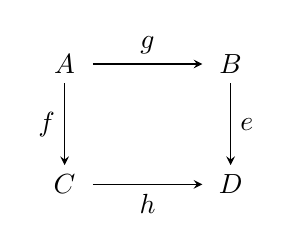
\begin{tikzpicture}
\matrix (m) [matrix of math nodes,row sep=3em,column sep=4em,minimum width=2em]
  {
     A & B \\
     C & D \\
  };
  \path[-stealth]
    (m-1-1) edge node [left] {$f$} (m-2-1)
            edge node [above] {$g$} (m-1-2)
    (m-2-1.east|-m-2-2) edge node [below] {$h$} (m-2-2)
    (m-1-2) edge node [right] {$e$} (m-2-2);
\end{tikzpicture}
\end{center}
\caption{Example of a commutative diagram}
\end{figure}

\begin{figure}
\begin{center}
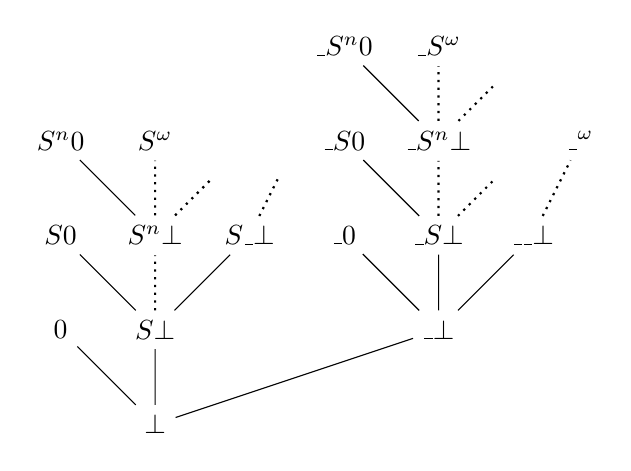
\begin{tikzpicture}
 [ grow'=up
 , scale=1.2
 , level distance=1cm
 , level 1/.style={sibling distance=3cm}
 , level 2/.style={sibling distance=1cm}
 , normal/.style={thin, solid}
 , skipping/.style={thick, dotted}
 , and so on/.style={thick, dotted, sibling distance=0.6cm, level distance=0.6cm}
 ]
  \node {$\bot$}
    child [sibling distance=1cm] { node {$0$} }
    child
    {
      node {$S\bot$}
      child { node {$S0$} }
      child [skipping]
      {
        %node {$SS\bot$}
        %child { node {$SS0$} }
        %child [skipping]
        %{
          node {$S^n\bot$}
          child [normal] { node {$S^n0$} }
          child [skipping] { node {$S^\omega$} }
          child [and so on] {}
        %}
        %child [and so on] {}
      }
      child
      {
        node {$S\_\bot$}
        child [missing] {}
        child [and so on] {}
      }
    }
    child
    {
      node {$\_ \bot$}
      child { node {$\_0$} }
      child
      {
        node {$\_S\bot$}
        child { node {$\_S0$} }
        child [skipping]
        {
          node {$\_S^n\bot$}
          child [normal] { node {$\_S^n0$} }
          child { node {$\_S^\omega$} }
          child [and so on] {}
        }
        child [and so on] {}
      }
      child
      {
        node {$\_\_\bot$}
        child [missing] {}
        %child [missing] {}
        child [skipping] { node {$\_^\omega$} }
      }
    }
  ;
\end{tikzpicture}
\end{center}
\caption{The domain $(Z, \sqsubseteq)$.}
\label{figDomainOfNuF}
\end{figure}

\begin{figure}
\begin{center}
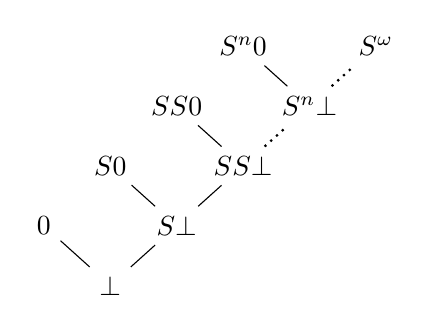
\begin{tikzpicture}[scale=1.2]
  \node {$\bot$} [grow'=up, sibling distance=4.0em, level distance=1.8em]
    child { node {$0$} }
    child
    {
      node {$S\bot$}
      child { node {$S0$} }
      child
      {
        node {$SS\bot$}
        child { node {$SS0$} }
        child [thick, dotted]
        {
          node {$S^n\bot$}
          child [thin, solid] { node {$S^n0$} }
          child { node {$S^\omega$} }
        }
      }
    }
  ;
\end{tikzpicture}
\end{center}
\caption{The domain of $L$, the lazy natural numbers.}
\label{figDomainOfLazyNaturals}
\end{figure}


\section{Further directions}

\section{Bibliographic notes}

This work is based on chapter 7 of the PhD thesis of Venanzio Capretta
\cite{Capretta2002}, where coinductive natural numbers are discussed.  Some
treatment of lazy natural numbers can be found in \cite{Escardo1993}.

A short introduction to denotational semantics can be found in
\cite{Allison1986}, while \cite{Gunter1992} is a more comprehensive treatment of
that topic.  A view on domain theory and denotational semantics from the
perspective of category theory can be found in \cite{Pierce1991},
\cite{Bird1997}, \cite{Mitchell1996} and \cite{BarrWells1990}.


\bibliographystyle{plain}
\bibliography{computer_science}
\end{document}

% vim: textwidth=80:spell:spelllang=en_us
